\chapter{Solution Proposed}\label{chap:4}

\section{Description}\label{sec:chap4_desc}
The system developed uses several elements in conjunction to work correctly, the core of the system is the actual AI, which has the name of Sam as it offers a unisex way of talking with the chatbot. In this chapter we will go into detail on how the system has been built and how the different elements provide the support for the different features the bot has.\\
The objective of this system is to create a simple way of tracking your progress, create dynamic tables which learn from you and provide a correct assessment and guidance to reach the users objective. The following points reflect what a final solution features would be:\\

\begin{itemize}
	\item{\textbf{Diet table creation:} Like the exercise table, this diet table would be based on what objective the user wants to reach. The bot will also consider what allergies the user may have and try to progressively adapt the table in order to transition from the user’s normal diet to the new diet without altering it all at once.}
	\item{\textbf{Training sessions:} This is a feature that could be added in the future if the speech technology keeps improving, as it would be ideal to have headphones on while Sam guides the user through the training session, this would make the user use less the phone and still keep track of brake times.}
	\item{\textbf{Gym location:} If a gym franchise or a multiple gym service bought the application this feature could make it easier for the user to find a gym nearby or maybe check what gyms are available at a certain location.}
	\item{\textbf{Exercise tutorials:} This could be a very useful functionality to make it easier for the user to know how to do an exercise, as some exercises by name may be confusing and this will make it easier to find out, compared to looking for it online.}
	\item{\textbf{Progress tracking:} With this the bot and the user can have an idea of how the training sessions is progressing, based on the results from the users measurements  the bot may choose to change the users diet, exercise table or remind the user to follow the diet table given.
		\begin{center}
			\begin{figure}[h!]
				\centering
				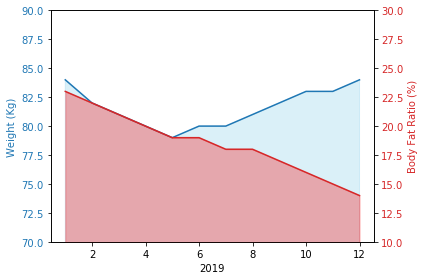
\includegraphics[scale=0.7]{./images/4-weight-bfr}
				\caption{User Weight vs Body Fat Ratio}
				\label{weight_bfr}
			\end{figure}
		\end{center}
	}
	\item{\textbf{Exercise table creation:} The bot provides new tables every month or may change if it sees throughout the month very little progress from the user. This table would be designed to fulfill the objective the user wants.
		\begin{center}
			\begin{figure}[h!]
				\centering
				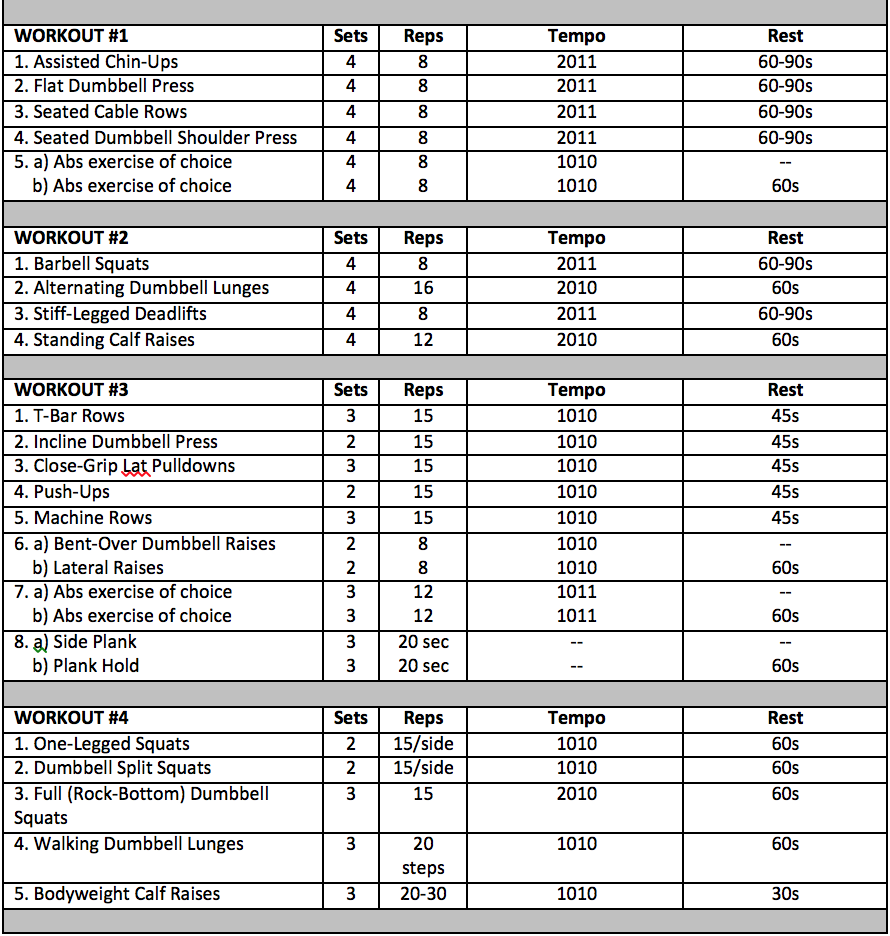
\includegraphics[scale=0.3]{./images/4-exercise-routine}
				\caption{Exercise Routine}
				\label{4_exercise_routine}
			\end{figure}
		\end{center}
	}
	\item{\textbf{Route recommendations:} At the moment the core functionality is based on gym training, especially weight lifting, but an interesting functionality that could be added in the future is for outdoor bike and running routes. With recommendations from users on the best routes.}
	\item{\textbf{Team meetings:} This functionality focuses on the social part of training, where users can arrange team matches between the users in what interest them more, even if the user’s interests are outdoor training or cycling teams, where they can arrange a route up a mountain, this will provide a community feeling in the application.}
\end{itemize}

\subsection{Reason for Building the Application}\label{sec:chap4_reas_app}

To prove that the application has a market opportunity an inquire was made to a group of people with over 200 people, the results where interesting as will be explained below. The language of the form is in Spanish as the public inquired live in Spain.\\

As shown below most of the users filling the form are from age 16 to 25, this gives context to some of the answers given afterwards, in this case generational mentality plays an important role as different age groups may have a different opinion on gym training. In this case the target group even though available for every age group is more focused on people in those age limits as they are the most common at gyms, the least informed and the more friendly with technology they are.

\begin{center}
	\begin{figure}[h!]
		\centering
		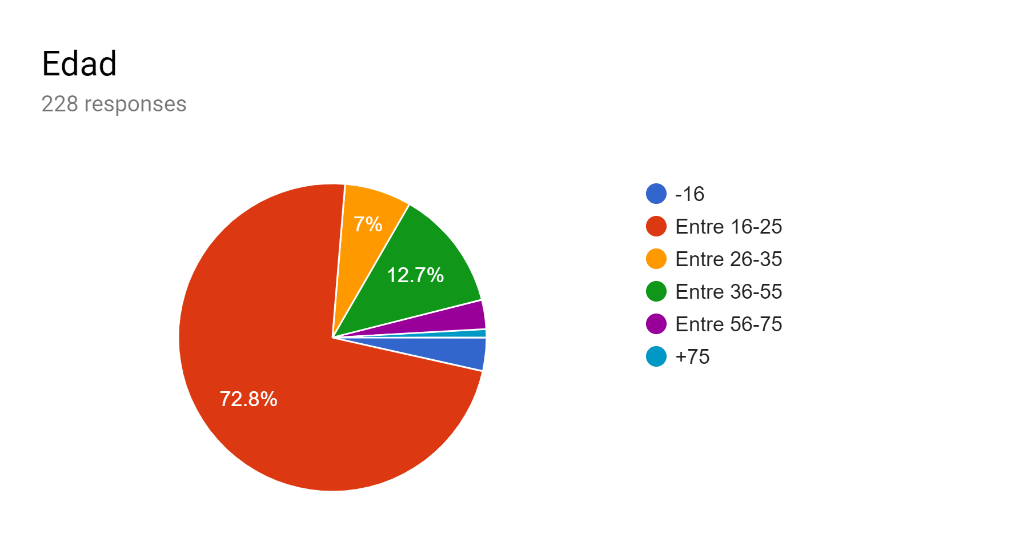
\includegraphics[scale=1]{./images/4-age}
		\caption{Survey: Age}
		\label{4_age}
	\end{figure}
\end{center}

In the case of gender, the pool has been varied with close to 50\% of each gender, this with the age group gives a general perception of what people think of the questions asked.

\begin{center}
	\begin{figure}[h!]
		\centering
		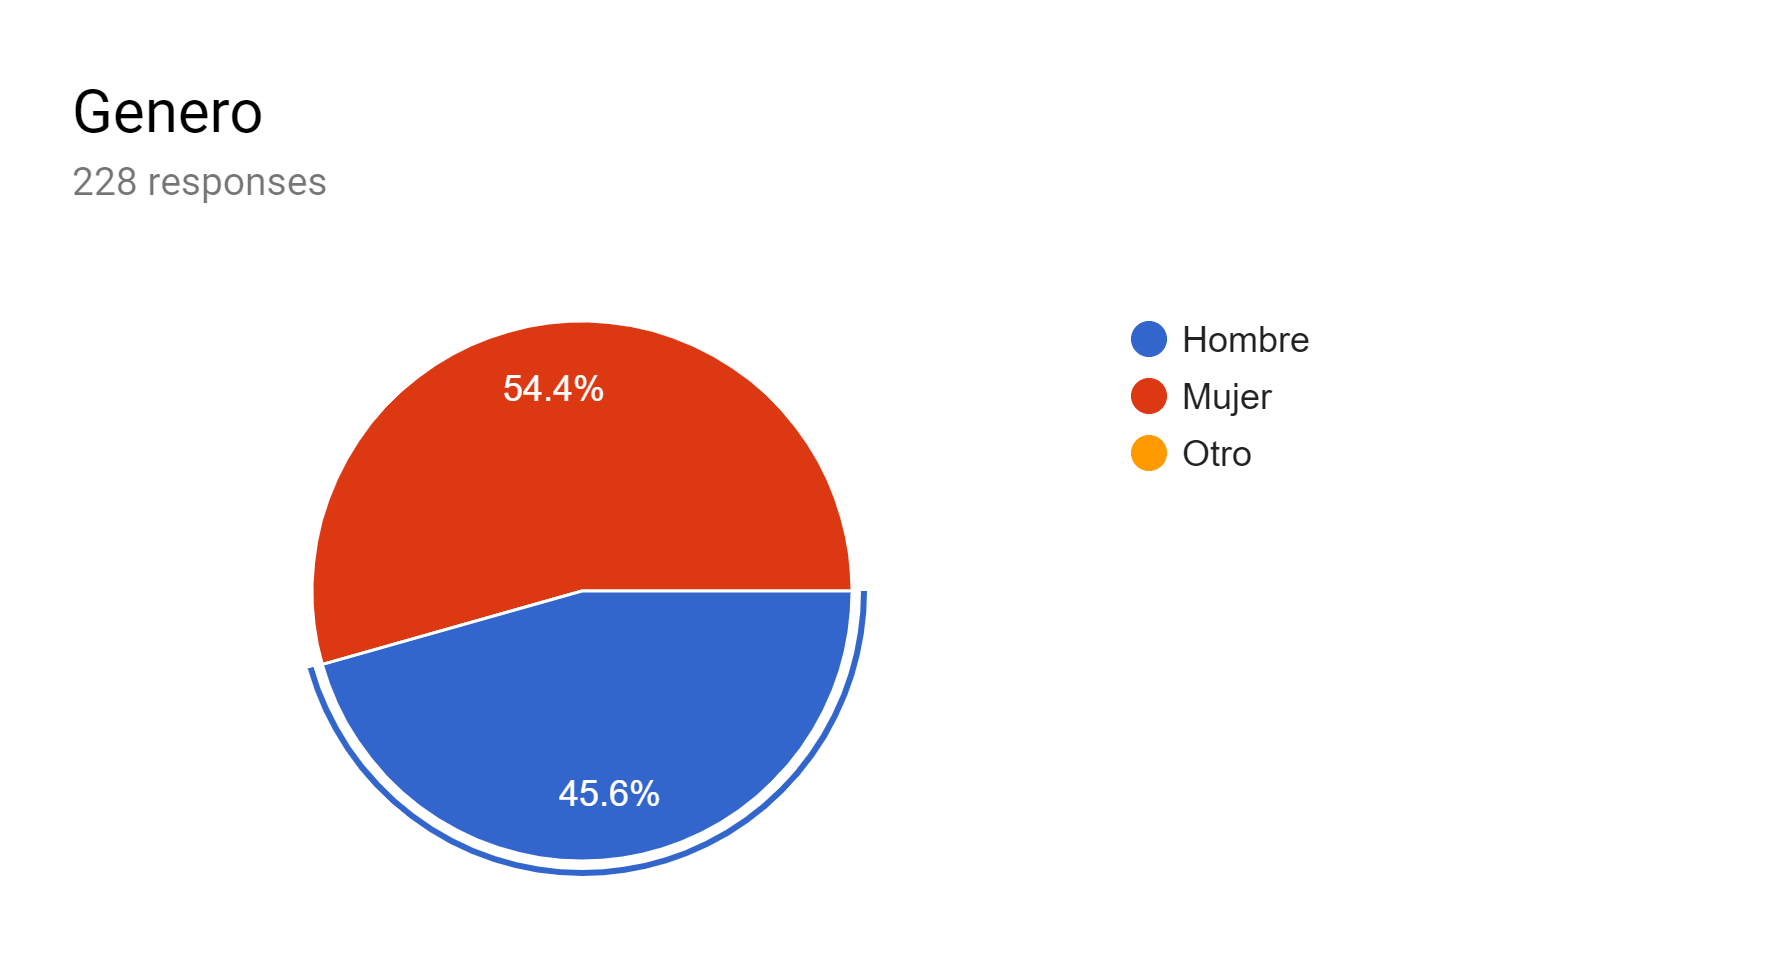
\includegraphics[scale=0.25]{./images/4-genero}
		\caption{Survey: Gender}
		\label{4_genero}
	\end{figure}
\end{center}

The following graph starts to show some interesting results, we can see that 30\% of the people asked don’t do any type of training and a sum of 24,1\% only train one to two times a week, this isn’t unexpected but that is over 50\% of people that train below the recommended amount weekly.

\begin{center}
	\begin{figure}[h!]
		\centering
		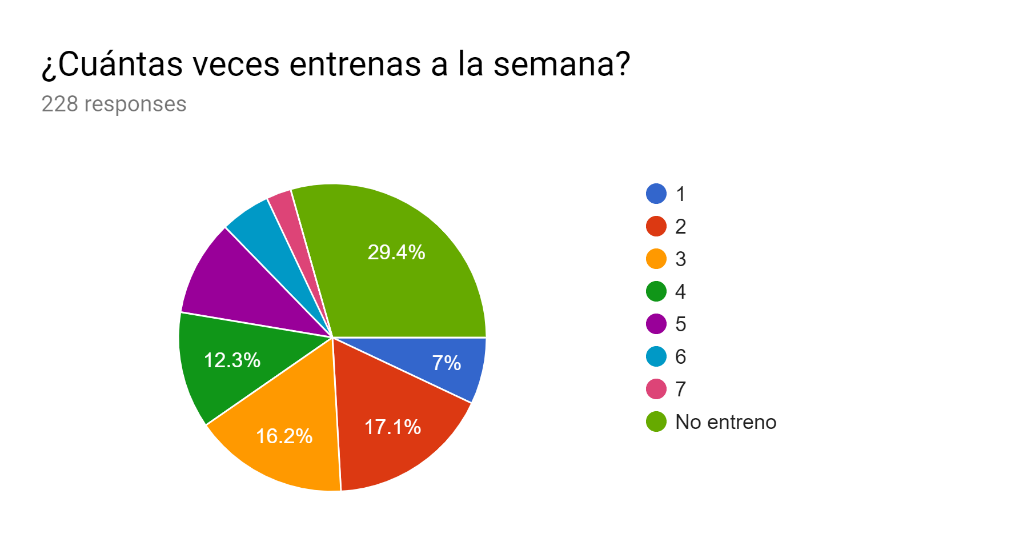
\includegraphics[scale=1]{./images/4-exe-freq}
		\caption{Survey: Gym Frequency}
		\label{4_exe_freq}
	\end{figure}
\end{center}

In the next graph the conclusions we can extract is that from the people that did the survey 30,7\% follow their own knowledge when going to the gym, this is something that is very frequent in gyms and it is the main source of dropouts as many people that follow what they know don’t actually have the required knowledge to do so. Another point we can extract from here is that 11,4\% use tables while training, this could provide a potential group to focus the bot to. The inconvenient part of information we can extract is that people don’t usually use applications when they train, so in order to reach the audience, the bot must seem as human as possible.

\begin{center}
	\begin{figure}[h!]
		\centering
		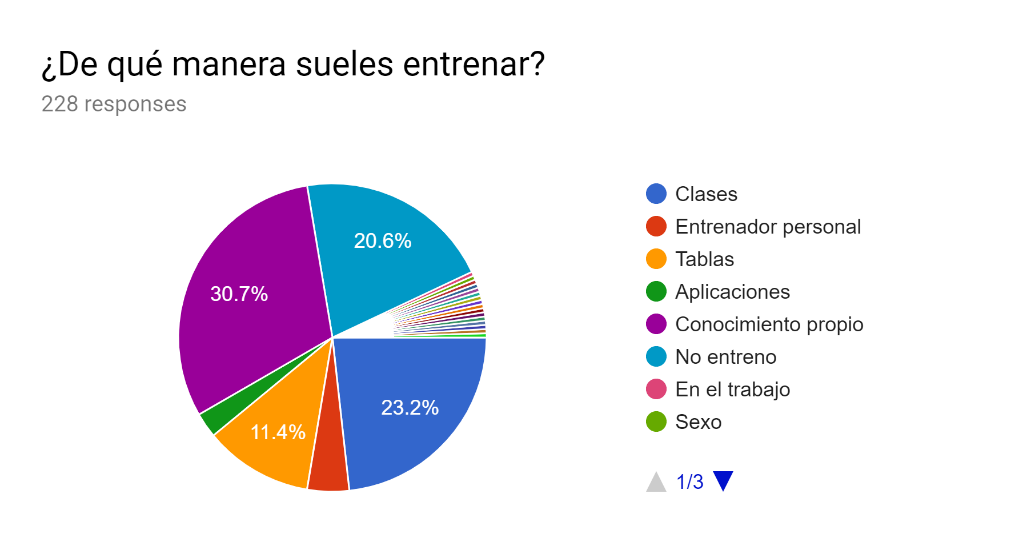
\includegraphics[scale=1]{./images/4-train-type}
		\caption{Survey: Training Type}
		\label{4_train_type}
	\end{figure}
\end{center}

The following pie represents if a personal trainer would motivate a user to go to the gym more often, this was surprising, as over 50\% would be motivated to go to the gym if they had a personal trainer guiding them and 34,2\% would maybe feel motivated to do so, after analyzing the previous graphs we consider that there is a market for a personal trainer application.

\begin{center}
	\begin{figure}[h!]
		\centering
		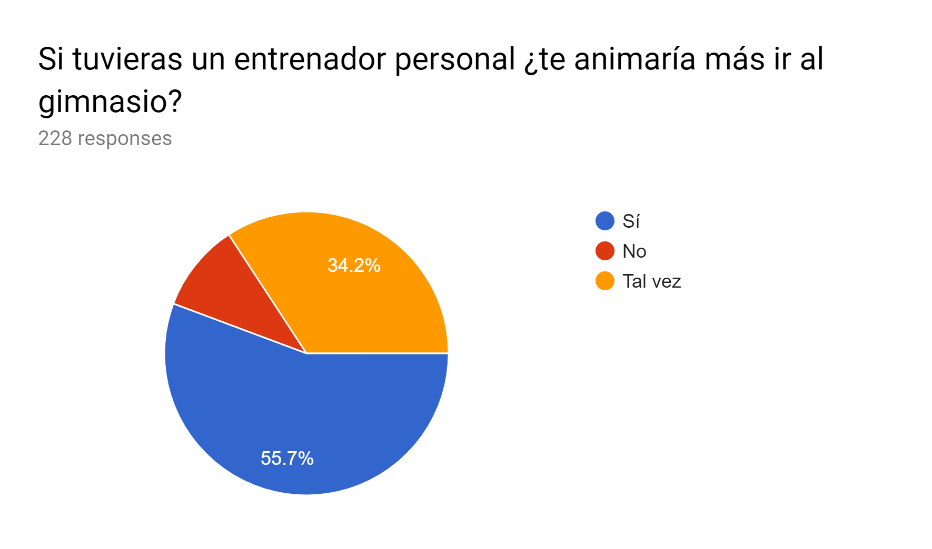
\includegraphics[scale=1]{./images/4-if-trainer}
		\caption{Survey: Having a Trainer}
		\label{4_if_trainer}
	\end{figure}
\end{center}

In the chart below we can extract some conclusions from the data, we think that 64\% of users change in some way the way they eat when they start training, but most don’t follow a strict diet. This is an important factor when developing the bot as the functionality for the recommended diets can be adapted to provide diets which tries to follow the most common eating habits of the user and slowly transition to a stricter diet, this will make users less prone to not following it.

\begin{center}
	\begin{figure}[h!]
		\centering
		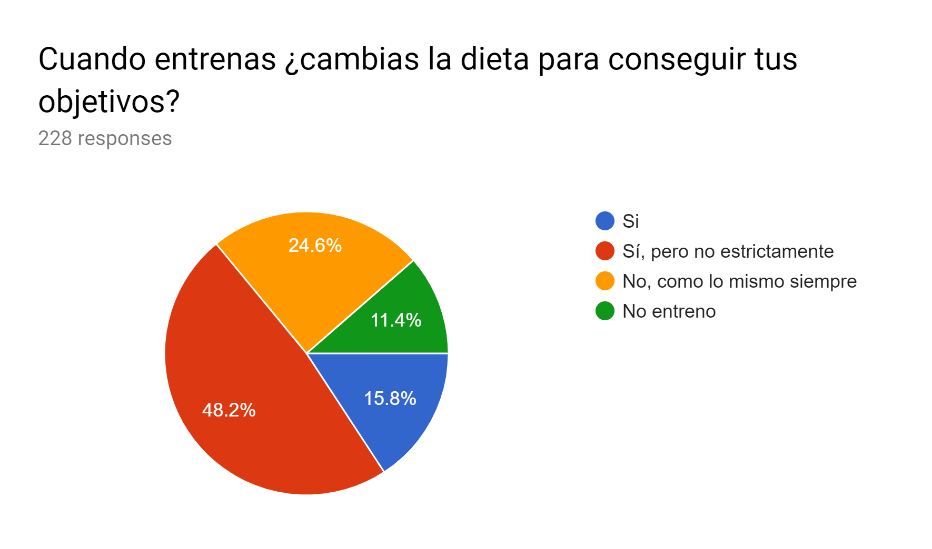
\includegraphics[scale=1]{./images/4-change-diet}
		\caption{Survey: Diet Change}
		\label{4_change_diet}
	\end{figure}
\end{center}

This graph follows up with the previous one and supports the conclusion extracted, that users rather have someone assisting with what meals to recommend the user with 84,6\% that would follow a diet recommended to them.

\begin{center}
	\begin{figure}[h!]
		\centering
		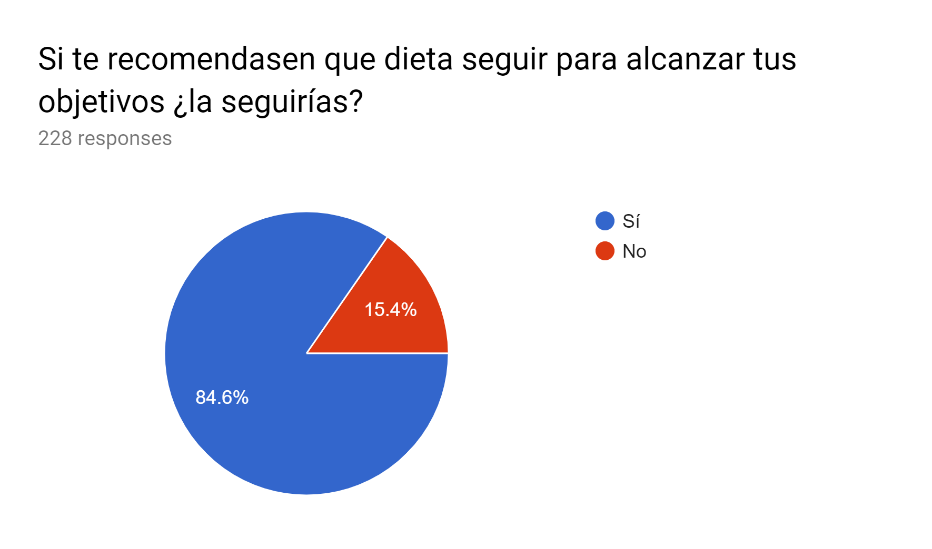
\includegraphics[scale=1]{./images/4-diet-rec}
		\caption{Survey: Diet Recommendation}
		\label{4_diet_rec}
	\end{figure}
\end{center}

The same as the previous chart in relation to exercises, the public is open and prefer someone guiding them to reach their objectives, in this case regarding exercises. This has to do with people using their own knowledge to train as compared to this graph some of the people that followed their own knowledge would rather have some one recommend what exercises to do.

\begin{center}
	\begin{figure}[h!]
		\centering
		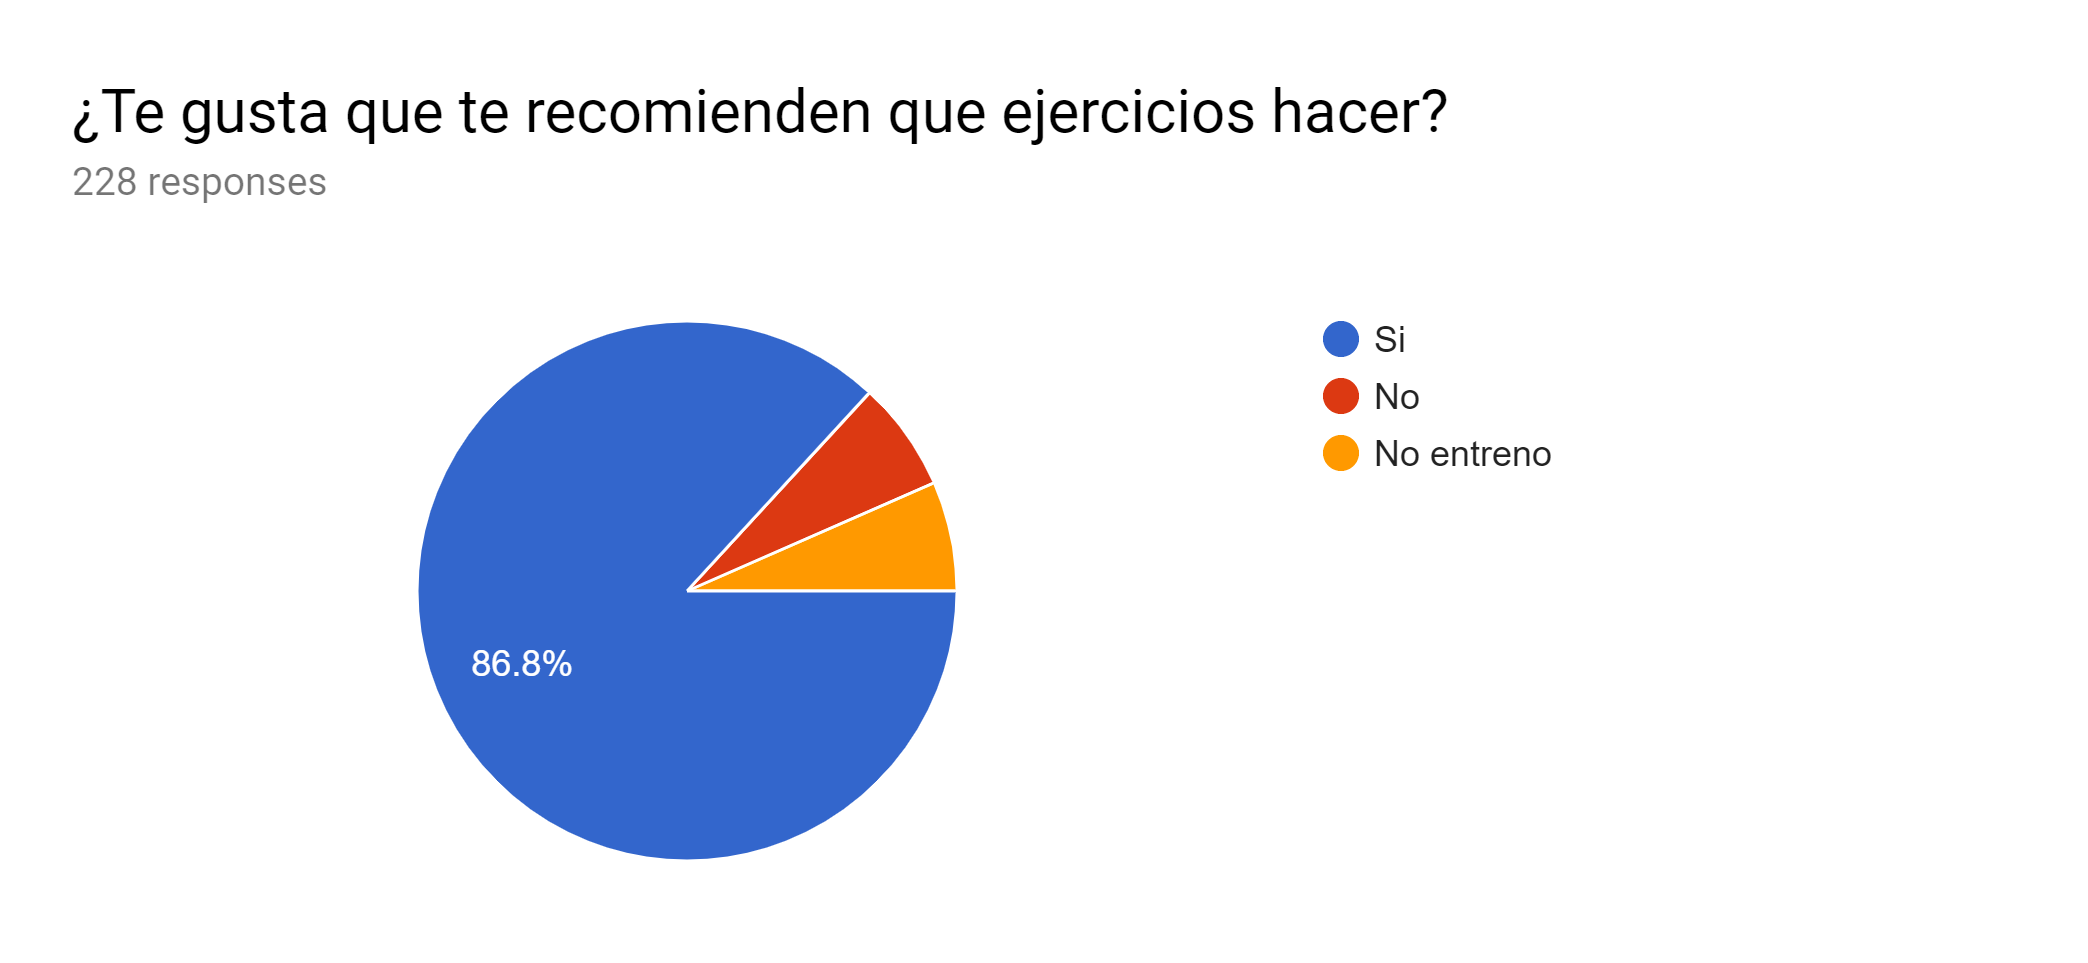
\includegraphics[scale=0.25]{./images/4-rec-exe}
		\caption{Survey: Exercise Recommendation}
		\label{4_rec_exe}
	\end{figure}
\end{center}

The most important chart of all is regarding our application, which is if these recommendations where given by a chatbot, if they would still follow it. Some curious points can be extracted from this pie, which are that most people would rather hire a professional trainer, what this tells us is that many people still prefer human contact over having a bot telling them what recommendations to follow, another point which links to a previous graph where we talked about how people train is that only 4.1\% have personal trainers, the reason being that hiring a personal trainer is costly so considering that and the fact that 35,1\% of people would follow those recommendations gives the application a large market to focus to, but also implies that the chatbot must try and simulate a human being as good as possible.

\begin{center}
	\begin{figure}[h!]
		\centering
		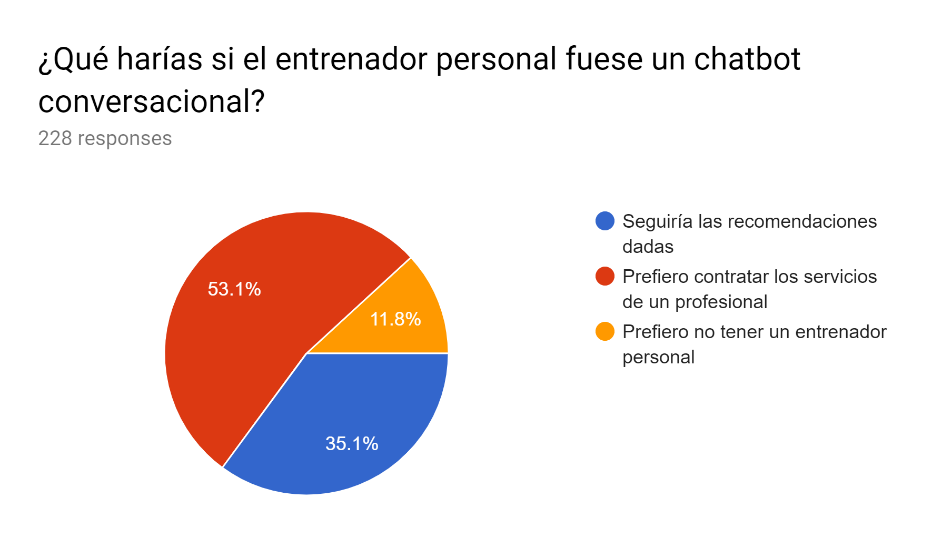
\includegraphics[scale=1]{./images/4-bot-trainer}
		\caption{Survey: Bot Trainer}
		\label{4_bot_trainer}
	\end{figure}
\end{center}

\section{Design}\label{sec:chap4_design}

In this project we find that there has been two different designs, the original design was developed in a way to make the system homemade, without depending on an external platform which even though it provides a base where to start developing it limits the control the developer has in adding new functionality.\\

The second and final design does use an open source platform as the base to start developing, this had to be done because of the complexity related in developing the proprietary solution in relation to the time available to develop it. Further down the memory the reason for changing the design will be explained in more detail.

\subsection{Original Design: Frontend}\label{sec:chap4_ori_des_front}

\begin{center}
	\begin{figure}[h!]
		\centering
		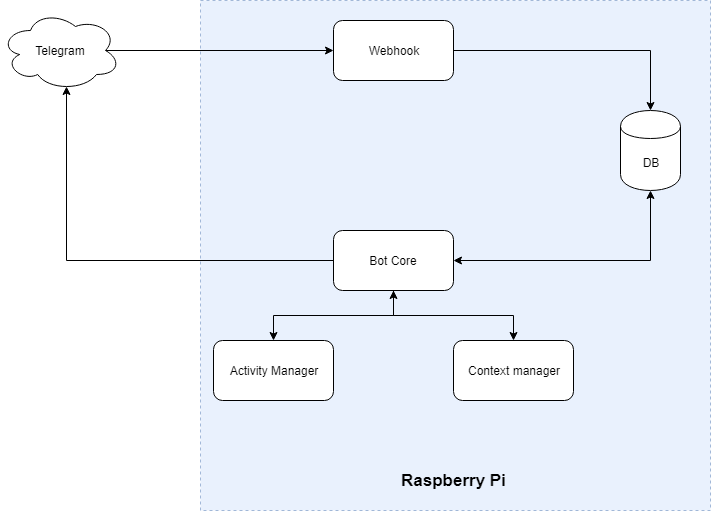
\includegraphics[scale=0.5]{./images/4-original-struct}
		\caption{High Level Original Design}
		\label{4_original_struct}
	\end{figure}
\end{center}

Following a model view controller architecture, the project uses as the view part Telegram, a chat platform for the users to contact the bot. The bot can be ported to different chat platforms based on preferences from the users, the reason Telegram was chosen instead of another platform where:

\begin{itemize}
	\item{\textbf{Higher user count:} Compared to Slack, another chat platform with support for bots, Telegram had for the year 2018, 200 million active users, while Slack only has 10 million. The reason to choose a chat platform with a higher count for active users is because with more users it is easier to penetrate the market. As the graph shows below it is also important that Telegram has been steadily growing in recent years with an increment of 100\% in one year from 100 million to 200 million active users.
	\begin{center}
		\begin{figure}[h!]
			\centering
			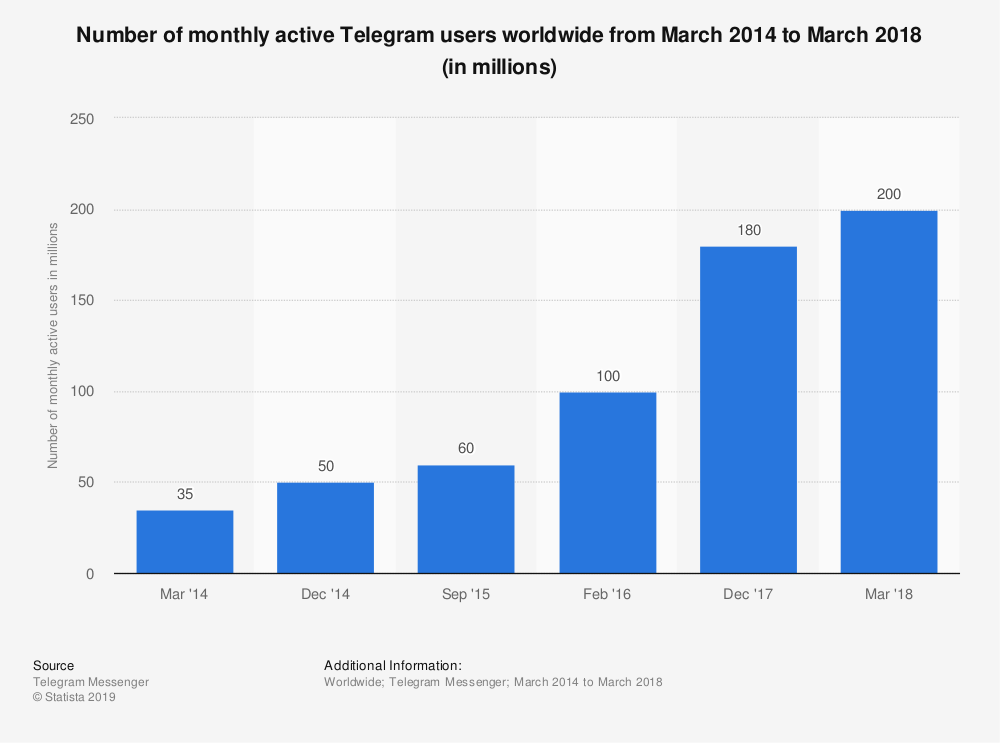
\includegraphics[scale=0.4]{./images/4-tele}
			\caption{Telegram User Growth}
			\label{4_tele}
		\end{figure}
	\end{center}
	}
	\item{\textbf{API:} Telegram has a very well documented API which makes it easier to integrate with the bot, also with previous knowledge in developing with Telegram it was the logical choice to use.}
	\item{\textbf{Webhook:} It provides a way of creating a bridge between Telegram servers and the Raspberry Pi to reduce stress at the network as Telegram automatically sends messages to the server instead of relying on the Raspberry Pi, polling Telegram servers.}
\end{itemize} 

\subsubsection{Webhook}\label{sec:chap4_ori_webhook}

After analyzing options to get the messages from Telegram, it was decided for this design to have a webhook instead of polling the server. A webhook is the bridge for communicating with the Raspberry Pi allowing to relieve the network from redundant traffic. The way a webhook works is like a web server which Telegram calls it whenever a message is received from a user. Whenever the webhook receives the message, it stores it in the database where the bot can check if anything new has arrived, this allows to transfer the stress from the network to the pc which reduces latency when receiving messages as polling a server takes longer than polling a database.

\subsection{Original Design: Backend}\label{sec:chap4_ori_des_back}

As the frontend was mostly managed by Telegram there wasn’t much to design except the webhook to support the message delivery.\\

For the backend we find the controller and the model for the bot. The way this two were designed is in that the controller was the communicator, were it managed the database where it extracted the user’s data two give back to the functions that performed the tasks. The first thing the controller does when getting a message from the database is authenticate the user, this is done with the telegram id sent from telegram, this id is unique to each user which makes it secure to identity fraud, at least from the applications end.\\
 
Below is the original flow for a message sent by the user to the bot, the design is at a high level to see where the message goes through until it gets to the response.

\begin{center}
	\begin{figure}[h!]
		\centering
		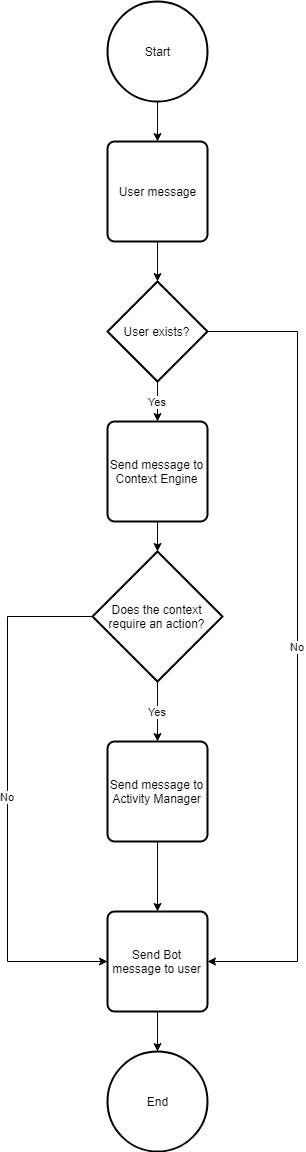
\includegraphics[scale=0.4]{./images/4-main-flow-ori}
		\caption{Main Flow Original Design}
		\label{4_main_flow_ori}
	\end{figure}
\end{center}

The flow follows starts once the message is grabbed from the database, the first thing is to verify that Sam is talking to a user from the platform, the idea is that the user doesn’t belong to the platform Sam offers to join the club. The complex part of the application was the context engine side of it.

\subsubsection{Context Manager}\label{sec:chap4_ori_cont_man}

The context engine is an engine which objective is to give the bot context from the user, this gives intelligence to the bot as it can remember what has been talked before. It also has the function of extracting data from what the user’s message. The following flow shows how it is intended to work. These are the main design objectives when creating the context engine.
\begin{itemize}
	\item{Being able to complete actions without following the happy path structure, in other words, if the bot wants to add measurements and there are two different measurement types there isn’t one way to provide those measurements, the user can facilitate them in several ways.
	\begin{itemize}
		\item{\textbf{I want to measure myself:} In this case the bot then will ask for the user’s weight.}
		\item{\textbf{Sam please add 80 kg as my new measurement and my current body fat ratio is 19\%:} In this case the context engine will extract both variables and delete the context as all relevant data has been extracted.}
		\item{\textbf{Sam my new body fat ratio is 19\%:} to which Sam will detect that the user has said its body fat ratio but not his weight and will ask the user to provide his weight as well.}
	\end{itemize}
	}
	\item{Keep the user in track whenever the user deviates from what is being asked.}
	\item{The context engine must be capable of extracting data correctly.}
	\item{Scalability is an important objective that the context engine must be designed for.}
	\item{The flows can be generated without having to manage code directly, the idea to make this work is to have the flows standardized as JSON formatted file. }
\end{itemize}

\begin{center}
	\begin{figure}[h!]
		\centering
		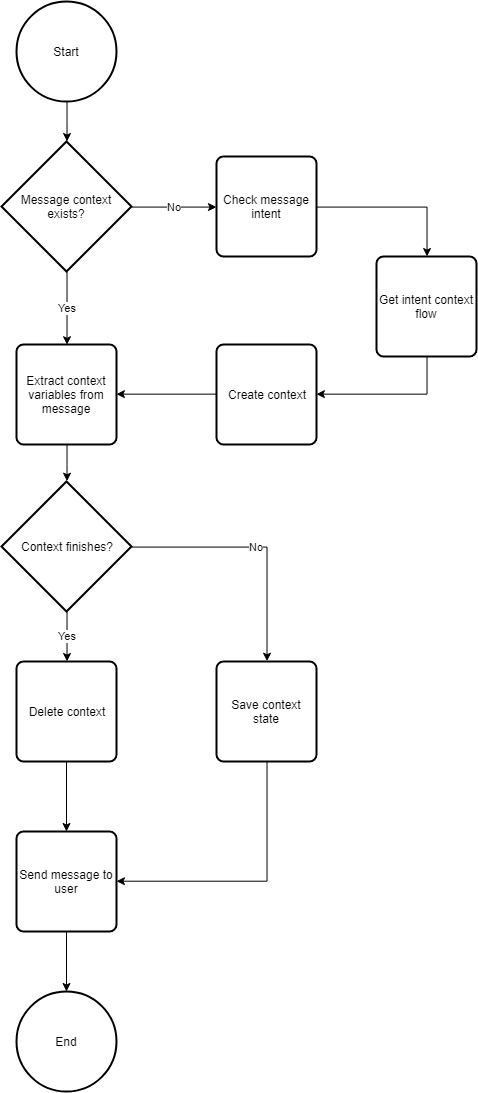
\includegraphics[scale=0.55]{./images/4-machine-learn-ori}
		\caption{Machine Learning Original Design}
		\label{4_machine_learn_ori}
	\end{figure}
\end{center}

\clearpage
\subsubsection{Activity Manager}\label{sec:chap4_ori_act_man}
The activity engine is the one in charge of performing the tasks required for the bot to be functional, the design is simple but the complexity in this manager is the functionality the developer wants Sam to have. The design for this is that it must be simple to add new functionality and not have to change to much code. The idea is to use the flows we talked about in the context manager section, in these flows if the context requires an activity to have the name of such activity in the JSON file and execute it in the activity manager.

\subsubsection{Scalability}\label{sec:chap4_ori_scale}
An important requirement for Sam is for him to be scalable, to reach this objective the architecture is designed in modules so that if a certain part of the application is receiving a higher level of stress to be able to scale it independently. This is done by having two masters, one for the activities and one for the context manager, these when launched by themselves act as a normal manager, but when several are launched acts as a load balancer.

\begin{center}
	\begin{figure}[h!]
		\centering
		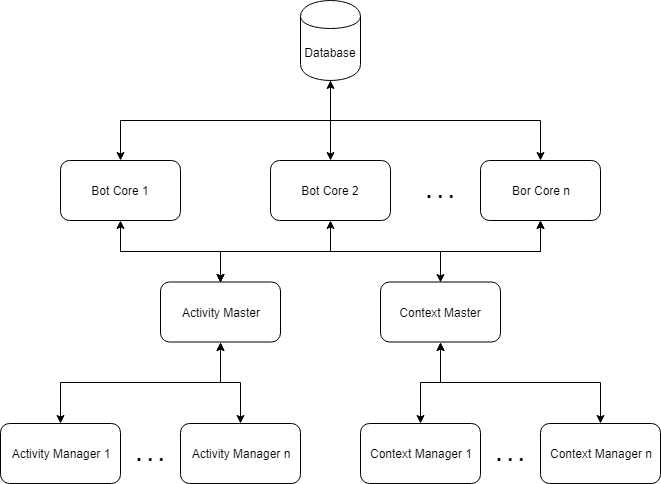
\includegraphics[scale=0.65]{./images/4-des-scal}
		\caption{Scalable Structure for Original Design}
		\label{4_des_scal}
	\end{figure}
\end{center}

\subsection{Final Design: Frontend}\label{sec:chap4_fin_des_fron}

For the final design the frontend only received some changes, the new design, as the original, still uses Telegram as the chat platform. One aspect that changed was the webhook, which for the revised version comes integrated with Rasa, so it doesn’t make any sense to develop it.

\subsection{Final Design: Backend}\label{sec:chap4_fin_des_fron}

As everything is designed following some rules, the changes the backend can have is limited to what Rasa offers.

\begin{center}
	\begin{figure}[h!]
		\centering
		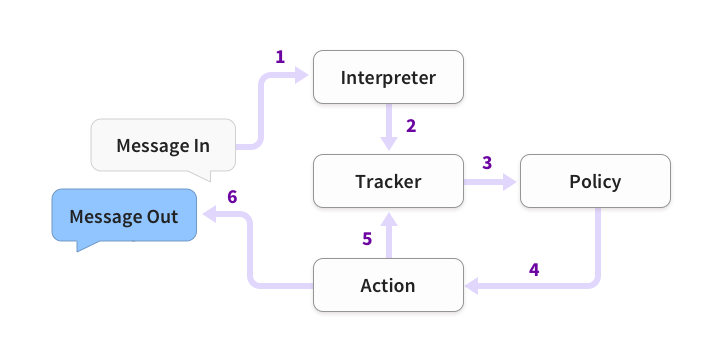
\includegraphics[scale=0.65]{./images/4-rasa-message-processing}
		\caption{Rasa High Level Structure}
		\label{4_rasa_message_processing}
	\end{figure}
\end{center}

The steps this new backend follows is different.

\begin{enumerate}
	\item {When a message is received it goes to the Interpreter, which in the original design would be part of the context manager, in the interpreter a dictionary is created which contains the original text, entities and the intent.}
	\item {An object linked to the state of the conversation called Tracker receives the info that a new message has arrived.}
	\item {The policy receives the state of the conversation with the user, this information comes from the tracker.}
	\item {Depending on the state the policy choses what action to take.}
	\item {The tracker logs the action taken from the bot.}
	\item {The response is sent back to the user.\cite{rasa-arch}}
\end{enumerate}

\subsubsection{Activity Manager}\label{sec:chap4_fin_act}

The activity manager has been changed because of the implementation of rasa, the way it has been designed is with what is called custom actions, which is similar in the way it was intended in the original design, but differs in the way it interacts with the data as it uses the database in conjunction with the Tracker from rasa which stores all the data extracted from the conversation.

\subsubsection{Story Manager}\label{sec:chap4_fin_stor}

The way that Rasa manages conversational chatbots is with the creation of stories. The stories are basically the flow of how the conversation is going to work as explained in section \ref{sec:chap3_rasa_core} in the state-of-the-art chapter. The advantage of this design compared to the original one is that it manages better deviations from the happy path, which is the correct way of completing a story. The disadvantage is that it requires a lot of training conversations for the bot to perform as intended, the design in the original had more restricted paths, so it was harder for the user to deviate from the original flow.

\subsection{Database}\label{sec:chap4_database}

The database remained the same for both designs as both required access to the same data. The design for the chatbot initially remains simple as the functionality to be developed for this proof of concept is limited. But the focus is around the individual user and with further development the addition of tables for groups and other more complex functionality may be added. Th use of a relational database was chosen as the preferred choice as the data’s integrity is relevant and queries are a must for this application.

\begin{center}
	\begin{figure}[h!]
		\centering
		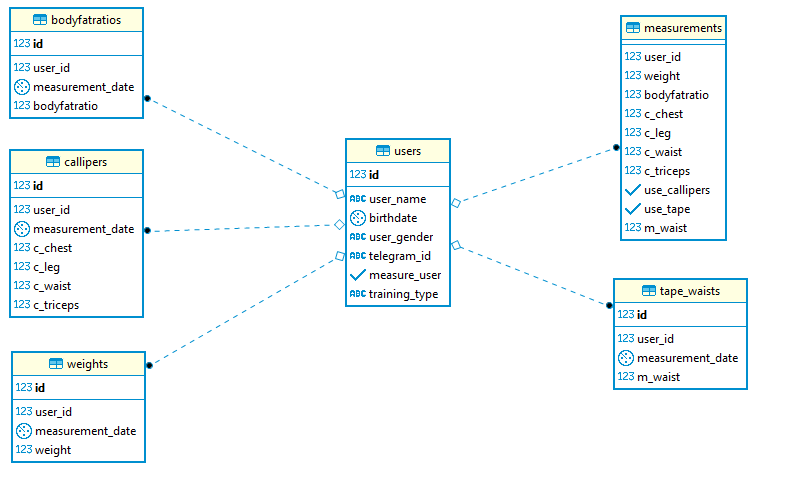
\includegraphics[scale=0.7]{./images/4-database-structure}
		\caption{Database structure}
		\label{4_database_structure}
	\end{figure}
\end{center}

The language to manage the database has been PostgreSQL as the team has had more experience developing in that language and the possibility of having more extensions than MySQL may offer a better option to have in the future.

\section{Resources Used}\label{sec:chap4_res_used}

\subsection{Hardware Resources}\label{sec:chap4_hard_res}

\begin{itemize}
	\item{Raspberry Pi to act as the server of the application, the brains of the chatbot, for more information check section \ref{sec:chap3_rasp}}
	\item{Azure as the cloud provider after porting the solution to the cloud, for more information check section \ref{sec:chap3_prov}}
	\item{Smartphone to test the bot and to use the application}
	\item{Laptop to develop the code and manage the server.}
\end{itemize}

\subsection{Software Resources}\label{sec:chap4_res_back}

\begin{itemize}
	\item {Python programming language}
	\item {Rasa Core for the second design, for more information check section \ref{sec:chap3_rasa_core}}
	\item {Atom, as the editor where the code is developed}
	\item {GitHub to keep track of the code}
	\item {NGINX to tunnel the web traffic received in the server to the correct port}
	\item {PostgreSQL as the SQL language to query the database, for more information check section \ref{sec:chap3_db}}
\end{itemize}

\section{Implementation}\label{sec:chap4_impl}
\subsection{Original Implementation}\label{sec:chap4_ori_imp}
\subsubsection{Webhook}\label{sec:chap4_ori_imp_web}

To develop the webhook first we had to prepare the Raspberry Pi to be able to act as a web server, as it was connected at home some management to the router had to be made in order to allow inbound traffic for HTTPS as this is the standard Telegram requires for the webhook to work. For it to be secure it was also required to create the certificates needed for SSL. These certificates where created with OpenSSL. Another issue that had to be solved in order for the webhook to work is have a domain name, the reason this is needed is because the network provider gives IP’s dynamically which caused Telegram to lose the connection whenever the IP’s was reset, initially a method was developed to automatically detect whenever the IP had changed, this was a very hacky way of solving the problem which resulted in some issues where the algorithm failed to update the SSL certificates which resulted in data loss and required human intervention to fix. To solve this problem a dynamic domain name provider by the name of \url{www.noip.com} provided a free DNS service which automatically updated the DNS whenever the IP had changed.\\

Once the Raspberry  Pi was set, it needed to have the web server running in order for it to work, below is the code for the API Rest that Telegram has to use in order to send the message to the server, has you can see once the message from Telegram is received it is stored in the database, this code can be expanded to support multiple platforms.

\begin{lstlisting}[language=Python]
from flask import Flask,request,abort
import json
import psycopg2

try:
	conn = psycopg2.connect("dbname='pt' user='matthew' host='localhost' password=***")
except:
	print ("ERROR: Unable to connect to the database")

app = Flask (__name__)

@app.route('/wbhk/tlgrm', methods=['POST'])
def webhook():
	if not request.json:
		abort(400)
	cur = conn.cursor()
	
	cur.execute("INSERT INTO webhook.incoming_messages (message, source) VALUES ('"+json.dumps(request.json)+"', 'Telegram')")
	
	conn.commit()
	cur.close()
	return json.dumps({'success':True}), 200, {'ContentType':'application/json'}
	
if __name__ == "__main__":
	app.run() 

\end{lstlisting}

\subsubsection{Controller}\label{sec:chap4_ori_imp_ctrl}

What the bot does at this stage is ask the database if any new message has been received, in order to make it scalable each bot has a unique id, this way whenever a bot gets a message from the database it can inform the rest of the bots what message is being worked on by which bot.\\
The bot after receiving the message sends it to the classifier through an API. Due to changing the implementation, the user detection wasn’t created, which would be used to identify if the user is in the system. After receiving the response from the context manager, it sends the response back to the user.\\
During the implementation of the original design the activity manager wasn’t built due to changing the whole model.

\subsubsection{Context Manager}\label{sec:chap4_ori_imp_manager}

When implementing the context manager, it was decided to create one predetermined flow for new users, this is done as we don’t want the user to have access to the rest of the flows. When developing the context manager, for the sprint being done the objective was to have the intent detected based on what the user says. This was done with the code below which follows these steps:

\begin{enumerate}
	\item {Stem the user’s phrase with NLTK’s Snowball stemmer}
	\item {After it converts the stemmed words into numbers.}
	\item {Then converts the count for the words into an array of the frequency in which the words appear in the training data.}
	\item {The different classifiers then predict what intent it is and take a vote on what intent it is, after that the result and probability that the prediction is correct is sent back to the user.}
\end{enumerate}

\begin{lstlisting}[language=Python]

def classify(data):
	if "text" not in data:
		abort(400)
	global threadLock
	array_statement = [data["text"]]

	array_statement = [" ".join([snow.stem(word) for word in sentence.split(" ")]) for sentence in array_statement]
	
	# thread lock
	threadLock.acquire()
	frases_new_counts = count_vect.transform(array_statement)
	frases_new_tfidf = tfidf_transformer.transform(frases_new_counts)
	
	vote = []
	pred_multi = multinomial_small_clf.predict(frases_new_tfidf)
	prob_multi = (multinomial_small_clf.predict_proba(frases_new_tfidf)[0][pred_multi[0]])
	vote.append(pred_multi[0])
	
	pred_sgdc = sgdc_small_clf.predict(frases_new_tfidf)
	prob_sgdc = (sgdc_small_clf.predict_proba(frases_new_tfidf)[0][pred_sgdc[0]])
	vote.append(pred_sgdc[0])
	
	pred_log = log_reg_small_clf.predict(frases_new_tfidf)
	prob_log = (log_reg_small_clf.predict_proba(frases_new_tfidf)[0][pred_log[0]])
	vote.append(pred_log[0])
	
	pred_lin = lin_svc_small_clf.predict(frases_new_tfidf)
	prob_lin = (lin_svc_small_clf.predict_proba(frases_new_tfidf)[0][pred_lin[0]])
	vote.append(pred_lin[0])
	
	pred_forest = forest_small_clf.predict(frases_new_tfidf)
	prob_forest = (forest_small_clf.predict_proba(frases_new_tfidf)[0][pred_forest[0]])
	vote.append(pred_forest[0])
	
	threadLock.release()
	prob_sum = prob_forest + prob_lin + prob_log + prob_sgdc + prob_multi
	prob_clf = (prob_sum)/5 * 100
	# thread unlock
	try:
		decission = mode(vote)
	except Exception as e:
	
		log("Two intents possible", LogTypes.LOG_WARNING)
		c = Counter([1, 1, 2, 2, 3])
		c.most_common(1)
		decission = c[0]
	
	confidence = (vote.count(decission)/len(vote)) * 100
	probability = (confidence + prob_clf)/2
	intent = intents[decission]
	print("Probability: ", probability, file=sys.stderr)
	print("Category: ", intent, file=sys.stderr)
	
	if probability > 70:
		json_msg = {'intent': intent,
					'sentence': data["text"]}
		new_entry(json_msg)
	
	result = {'intent_id': format(decission),
			  'intent': intent,
			  'probability': "{:.2f}".format(probability)}
	
	return json.dumps(result)


\end{lstlisting}

After reaching this objective, we started realizing that to finish creating the context manager would be to complex and being in the time constraint and haven’t developed any functionality for the personal trainer it was decided to change the platform to something higher level but with still the capability of modifying it to the objective of the bot. It was a hard decision but in order to finish in time the correct choice.

\subsection{Final Implementation}\label{sec:chap4_fin_imp}

For the final design most of the code done was scraped as it was already included in Rasa.

\subsubsection{Raspberry Pi to Azure}\label{sec:chap4_fin_rasp_azur}

When trying to use Rasa as the new engine in the Raspberry Pi it started failing as the architecture in Rasa is more resource heavy, so in order to develop the new design with the credits offered by Microsoft for being a student we ported everything to the cloud. For this we created a virtual machine where Sam will be running.

\subsubsection{Config}\label{sec:chap4_fin_conf}

The config file for Rasa is where the developer designs how the bot is going to be, in this case the pipeline follows a modified version of the pretrained\_embeddings\_spacy, check section \ref{sec:chap3_rasa_nlu}. The pipeline translates to the following steps.

\begin{enumerate}
	\item {First, the language to be processes is chosen, in our case it is English.}
	\item {After it goes through Spacy’s Natural Language Processor, where the user’s message is normalized.}
	\item {Then the message is tokenized with Spacy’s Tokenizer.}
	\item {After Spacy’s features for intent classification are added.}
	\item {The regex featurizer gets regular expressions defined in the training data.}
	\item {The CRFEntityExtractor uses conditional random fields to extract entities.}
	\item {EntitySynonym converts synonyms to a defined value, very useful to convert different ways to say something in a normalized form.}
	\item {After the intent is detected using the Sklearn Intent Classifier.}
	\item {After detecting the intent Spacy predicts with its entity extractor what entities need to be extracted, it uses the statistical BILOU transition model, it is pretrained so doesn’t require new data, it is very useful for extracting user’s names it is an addition to the predefined pipeline.}
	\item {Finally, the DuclingHTTPExtractor that is also an addition to the predefined pipeline, the reason to add this to the implementation is that it provides good entity extraction for time entities such as birthdays.}
\end{enumerate}

\begin{lstlisting}

language: en
pipeline:
- name: "SpacyNLP"
- name: "SpacyTokenizer"
- name: "SpacyFeaturizer"
- name: "RegexFeaturizer"
- name: "CRFEntityExtractor"
- name: "EntitySynonymMapper"
- name: "SklearnIntentClassifier"
- name: "SpacyEntityExtractor"
- name: "DucklingHTTPExtractor"
  url: "http://localhost:8000"
  dimensions: ["time","distance", "number"]
  timezone: "Europe/Madrid"

policies:
- name: MemoizationPolicy
- name: KerasPolicy
- name: MappingPolicy
- name: "FormPolicy"


\end{lstlisting}

Another important part of the config file are the policies Rasa follows in the flow of the conversation. The reason these for where chosen where for the following reasons.

\begin{itemize}
	\item {\textbf{Memoization Policy:} This policy just memorizes the conversations in the training data, if the conversation with the user is already in the training data the confidence is 1.0, but if the conversation doesn’t follow any story the result is 0.0.}
	\item {\textbf{Keras Policy:} As not always the user will follow the standard paths in the training data this policy uses a neural network to select the next action, so even if the previous policy gave a result of 0.0 the Keras Policy can still predict the correct action based on the mix of all the training data.}
	\item {\textbf{Mapping Policy:} Works with certain intents that only require a unique response and has no relation with the rest of the flow, whenever an intent is mapped to an action if the intent is detected the mapped action will run and after fallback to the normal predictions.}
	\item {\textbf{Form Policy:} As an extension to the Memoization Policy, this policy handles filling a set of variables with what is called Forms, if a form is detected than the form action will run until it has completed.}
\end{itemize}

\subsubsection{Custom Actions}\label{sec:chap4_cust_act}

This is where the all Sam’s functionality is stored, whenever it is required to do anything extra apart from answering with a message these custom actions come in handy.\\
An example of this custom action is whenever a user speaks with the bot, it first has to run the action of checking if the user actually is part of the application.\\
For this story:

\begin{lstlisting}

## Known user
* greet
- action_check_profile
- slot{"user_exists": true}
- slot{"user_name": "Matthew"}
- slot{"measure_user": true}
- slot{"user_gender": "male"}
- slot{"user_id": "1"}
- utter_greet


\end{lstlisting}

Whenever the bot detects that the user is greeting him the first thing to do figure out who that user is, this is done with “action\_check\_profile” which does the following.

\begin{lstlisting}[language=Python]

class CheckProfile(Action):
	def name(self):
		return "action_check_profile"

	def run(self, dispatcher: CollectingDispatcher, tracker: Tracker, domain: Dict[Text, Any]) -> List[Dict[Text, Any]]:

		db = Database.get_instance()
		user_exists, user_id, user_name, user_gender, measure_user = db.check_user_exists(tracker.sender_id)
		return [SlotSet("user_exists", user_exists),
			    SlotSet("user_name", user_name),
				SlotSet("measure_user", measure_user),
				SlotSet("user_gender", user_gender),
				SlotSet("user_id", user_id)]
				
\end{lstlisting}

The database action queries the database for the relevant data, as you can see the action sets the corresponding sets, these are required to give Sam the context of who the user is, in the case that the user doesn’t exist, Sam knows to follow a different story.

\begin{lstlisting}

## Unknown user
* greet
- action_check_profile
- slot{"user_exists": false}
- slot{"user_name": null}
- slot{"measure_user": false}
- slot{"user_gender": null}
- slot{"user_id": 0}
- utter_unknown

\end{lstlisting}

The useful thing about custom actions is that it has integrated a system of reminders, this can be used to set alarms for users to measure themselves or train.

\subsubsection{Conversation Logs}\label{sec:chap4_conv_logs}

Rasa doesn’t offer many logging tools but does offer the possibility of storing the Tracker information, this contains everything relevant to the conversation but mixed it shows every step the bot does while interacting with the user, in order to get conclusions and analyze the user’s information a data scrubber must be implemented. This can be developed at a further date.

\section{Testing}\label{sec:chap4_test}

The way the original implementation was test-driven which means that that everything is focused around the tests.

\subsection{Unit Tests}\label{sec:chap4_test_unit}

Tests where created for every new module of the bot before starting implementation, initially as it may seem obvious the tests failed as no code was written yet, the objective was to create tests that prove that the method was working and then create the method for it to pass the test. An example of this is the classifier test shown previously in this chapter, check section  \ref{sec:chap4_ori_imp_manager}.

\begin{lstlisting}[language=Python]

class TestClassifier(unittest.TestCase):

	def test_classify(self):
		tests = [
		('hello', 'salute'),
		('good morning', 'salute'),
		('hi sam', 'salute'),
		('good afternoon', 'salute'),
		('good bye', 'bye'),
		('bye sam', 'bye'),
		('see you later', 'bye'),
		('that will be all', 'bye'),
		('I need help', 'help'),
		('what can i do', 'help'),
		('what commands can i say', 'help'),
		('help', 'help'),
		('what is the weather', 'unknown'),
		('breakfast time', 'unknown'),
		('where is the closest shop', 'unknown'),
		('where can i watch the game', 'unknown'),
		('i would like to measure myself',
		'get_measurements'),
		('i want to measure myself', 'get_measurements'),
		('i want to weigh myself',
		'get_measurements'),
		('new measurements', 'get_measurements'),
		('configure a new table for me', 'new_table'),
		('create new table', 'new_table'),
		('i want a new table', 'new_table'),
		('can you send me a new table?', 'new_table'),
		("let's start training", 'start_training'),
		("i want to train", 'start_training'),
		('time to train', 'start_training'),
		('start training session', 'start_training')
		]
		
		for value, expected in tests:
		
			with self.subTest(value=value):
				# add call to classify funtion
				result = json.loads(classifier.classify({'text': value}))
				intent = result['intent']
				self.assertEqual(intent, expected)

\end{lstlisting}

Until this test passed the method was tweaked. This was done with every method of the application.

\subsection{Integration Tests}\label{sec:chap4_test_inte}

This as we explained in State of the Art section \ref{sec:chap3_test} helps the developer check if the different methods together work well together, this was going to be done for the integration of the context manager as it required several modules operating together but never was developed due to changing the design to Rasa.

\subsection{End-to-end Tests}\label{sec:chap4_test_end}

All end-to-end tests where done manually due to the simplicity of the bot at that stage, most tests where to verify that the webhook, the processor and the intent classifier were working well together. The plan was to create a simple bot to act as the user with predetermined conversations to verify that the bot could manage different types of conversation.